\chapter{Architettura Base della CPU}

\section{Architettura complessiva}

\begin{figure}[H]
    \centering
    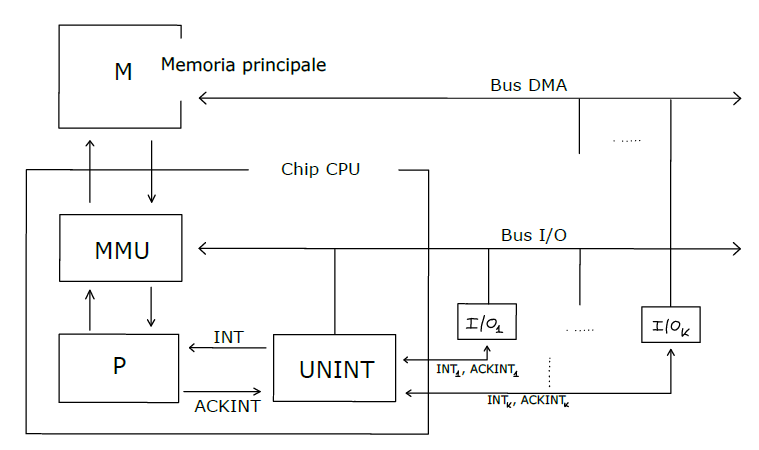
\includegraphics[width=\textwidth]{immagini/ArchitetturaBase.png}
\end{figure}

\noindent L'unità MMU, oltre che tradurre in maniera molto efficiente gli indirizzi logici, ha anche il compito più generale di interfacciare tutte le unità, svincolando il progetto del processore da molti aspetti legati alla realizzazione fisica della memoria nonché del sottosistema di I/O.

Tutte le unità di I/O usano il Bus di I/O per scambiare informazioni direttamente con il processore centrale; tali informazioni potranno essere \textit{dati} e/o \textit{comandi} che interessano la cooperazione tra processi centrali e unità di I/O.

Un certo sottoinsieme di unità di I/O può anche trasferire dati nei confronti dell'unità centrale accedendo \textit{direttamente in memoria} (\textit{DMA}: Direct Memory Access): è soprattutto il caso di unità (come dischi, stampanti veloci, unità di rete) che effettuano i trasferimenti a \textit{blocchi}, alleggerendo quindi notevolmente il processore dal compito di gestire il trasferimento, e quindi permettendo al processore stesso di eseguire parallelamente altri processi.\
Il \textit{Bus DMA} provvede a realizzare un canale diretto tra le unità di I/O e la memoria principale.

Le \textit{interruzioni} hanno un doppio significato:

\begin{itemize}
    \item \textit{a livello firmware}, sono segnali per il meccanismo di arbitraggio del Bus di I/O.\ Ogni volta che un'unità di I/O ha bisogno di segnalare eventi direttamente al processore, deve usare il Bus di I/O in scrittura e, quindi, deve prima interagire con l'arbitro di tale Bus attraverso dei segnali, detti appunto \textit{segnali d'interruzione};
    \item \textit{a livello dei processi}, partecipano a supportare la cooperazione e sincronizzazione tra i processi eseguibili dalla CPU ed elaborazioni concorrenti effetturare dall'unità di I/O.
\end{itemize}

\noindent All'interno della CPU, è l'unità indicata con UNINT che esegue le funzioni di arbitraggio vere e proprie.\
Anche in questo caso, la presenza di UNINT svincola il progetto del processore da tutta una serie di scelte implementative legate all'arbitraggio delle interruzioni; inoltre, tale arbitraggio avviene in parallelo all'elaborazioni del processore.

Il segnale d'interruzione INT, testato dal processore alla fine dell'interpretazione di ogni istruzione assembler è il risultato della funzione OR, realizzato in UNINT, di tutti i segnali d'interruzione.\
Nel caso accetti l'interruzione, il processore invia il segnale \texttt{ACKINT} a \texttt{UNINT}, la quale provvede a smistarlo all'unità prescelta dal meccanismo di arbitraggio.

\section{Interprete del set d'istruzioni}

\subsection{Specifiche della macchina firmware}

Oltre agli stessi registri assembler RG[0..63] e al registro IC, la macchina firmware contiene ovviamente
(nella PO del processore) altri registri, \textit{visibili solo a questo livello}, come:

\begin{itemize}
    \item IR: registro istruzione corrente;
    \item registri temporanei e interfacce.
\end{itemize}

\noindent La memorietta per implementare l'array RG consente, in uno stesso ciclo di clock, \textit{la lettura di due registri} e \textit{la scrittura in un singolo registro}.\
RG deve essere indirizzabile, oltre che dai campi di IR, anche dai campi di altri registri e costanti generati dalla PC.

\begin{figure}[H]
    \centering
    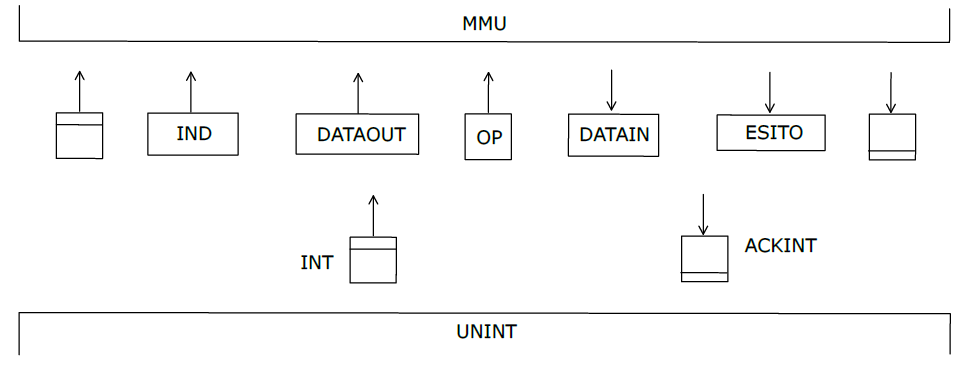
\includegraphics[width=\textwidth]{immagini/Interfaccia MMU.png}
    \caption*{Interfaccia a transizione di livello del processore verso la MMU e verso la UNINT}
\end{figure}
\begin{figure}[H]
    \centering
    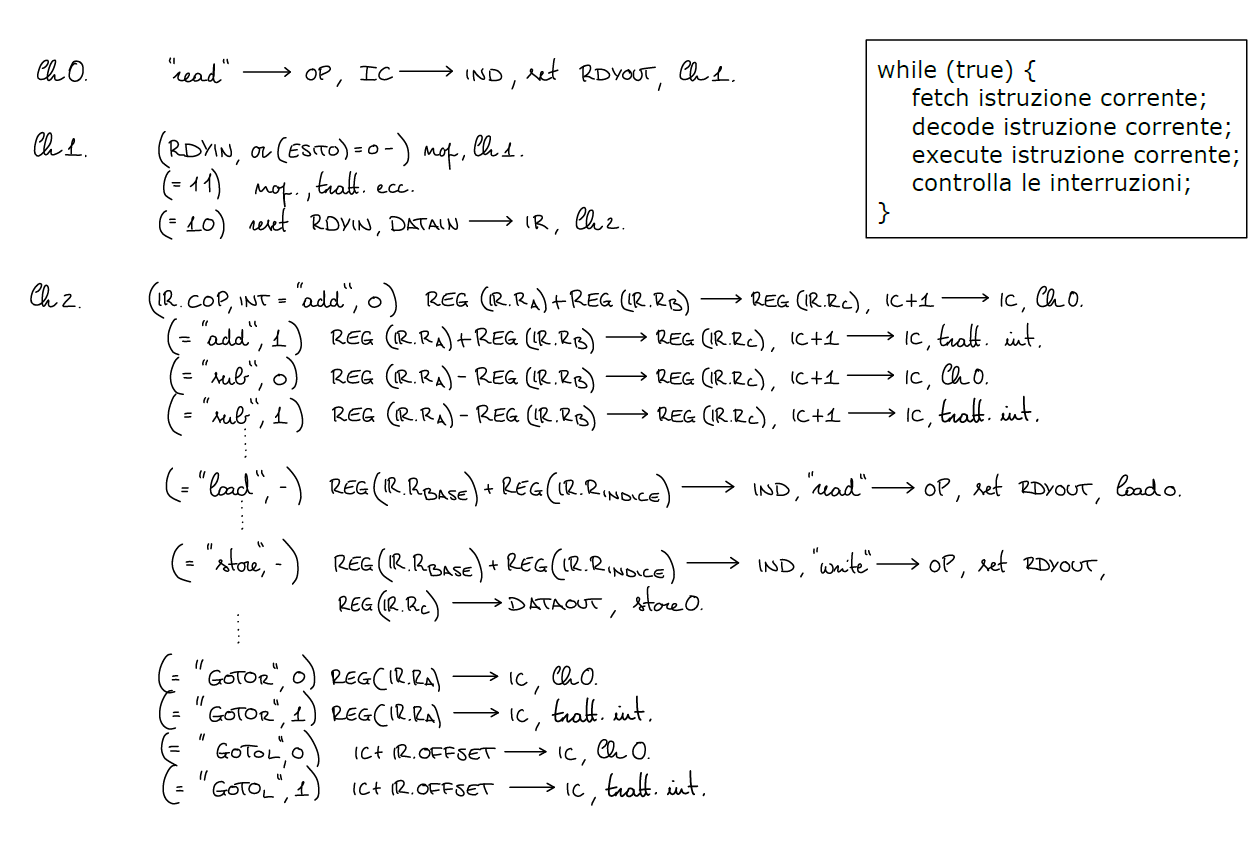
\includegraphics[width=\textwidth]{immagini/Interprete.png}
\end{figure}

